\documentclass[paper=a4, fontsize=11pt]{scrartcl}
\usepackage{amsmath,amsfonts,amsthm}
\usepackage{graphicx}
\usepackage{multirow}
\usepackage{hhline}
\usepackage{parskip}
\usepackage{hyperref}
\usepackage{chngcntr}

\newcommand{\horrule}[1]{\rule{\linewidth}{#1}}
\parskip = \baselineskip

\title{
	\normalfont \normalsize \textsc{THE PENNSYLVANIA STATE UNIVERSITY} \\ [25pt]
	\horrule{1pt} \\[0.4cm]
	\huge {\bf CSE585/EE555: Digital Image Processing II Report 1 \\ Mathematical Morphology} \\
	\horrule{2pt} \\[0.5cm]
}
\author{
	\normalfont \normalsize
	 Wei-Kai Su, Yu-Hsuan Kuo\\[-3pt] \normalsize
  \today
}
\date{}

\begin{document}
\maketitle

\section{Objectives}
This project is mainly focus on applying the hit-or-miss transform to detect three middle-size disks. The given binary-valued image considers WHITE to be background and BLACK to be foreground and with five different sized black disks scattered around. The objectives of this project 1 are listed as follows: 

\begin{itemize}
	\item Remove the 10\% level of salt-and-pepper noise.
	\item Threshold the input image to convert to a truly binary-valued image.
	\item Design an appropriate hit-or-miss transform $( X \ominus A^S) - ( X  \oplus  B^S)$

\end{itemize}



\section{Methods}

The flow of the project includes: noise removal, thresholding, pixel value inversion and  hit-or-miss transformation. We implemented two noise removal methods, and we get the same result from both of them. The results of these methods are discussed in the next section. And, the structure of our code is presented in $main.html$ file in html folder.
\subsection{Salt-and-Pepper Noise Filtering}

\subsubsection{Method 1 - Median Filtering}
First, we convert the image to grayscale image. Next, given that the image is corrupted by salt-and-pepper noise, we performed the median filter on our input image in the preprocessing step. The main idea of the median filter is to replace the value of a pixel by the median of the intensity values in the neighborhood of that pixel. The median filter is because its particularly effective in the presence of impulse noise (also called salt-and-pepper noise) because of its appearance as white and black dots superimposed on an image. Figure \ref{fig:1} demonstrates the result after median filtering. The detailed implementation is shown in the $medianFilt.m $ file.  %?However, during our implementation, we met a problem of image show. The reason is the data type of pixel values is unsigned, and after the operation in the our medianFilt() function, the data type of pixel values turned out to be double. Therefore, we converted the data type to unsigned to show the correct image. 

After the noise removal has been done, we conducted thresholding for generating binary-valued image. Our threshold value is set to be 200. This is because, we found out that, after the median filtering, the pixel value of the salt noise reduced (close to gray level 0) while the pixel value of the pepper noise increased (around the gray level 255). Therefore, if the pixel value is larger than 200, we reset the pixel value to 255 (White). Otherwise, we reset the pixel value to 0 (Black). In figure \ref{fig:2}, it shows the result after thresholding. The detailed implementation is shown in the $threholdv.m$ file.

\begin{figure}
	\centering
	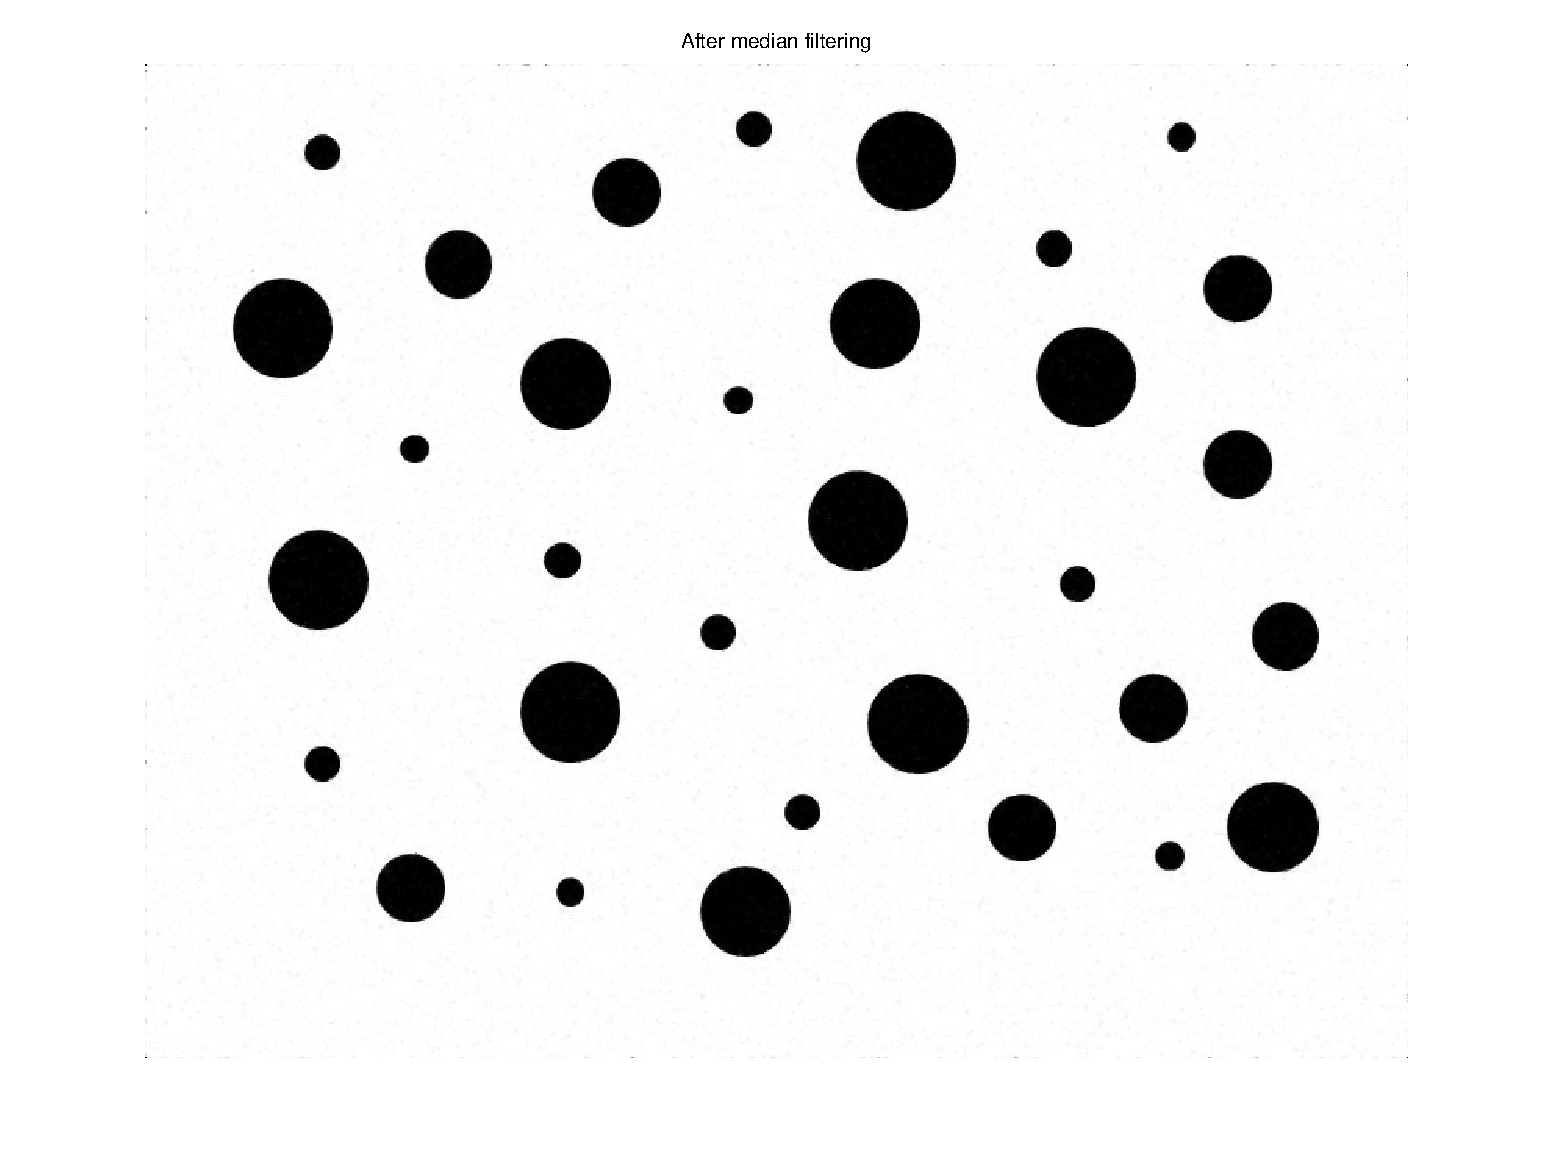
\includegraphics[width=12cm]{after_medianfiltering.eps}
	\caption{Median Filtering Result.}
	\label{fig:1}
\end{figure}


\begin{figure}
	\centering
	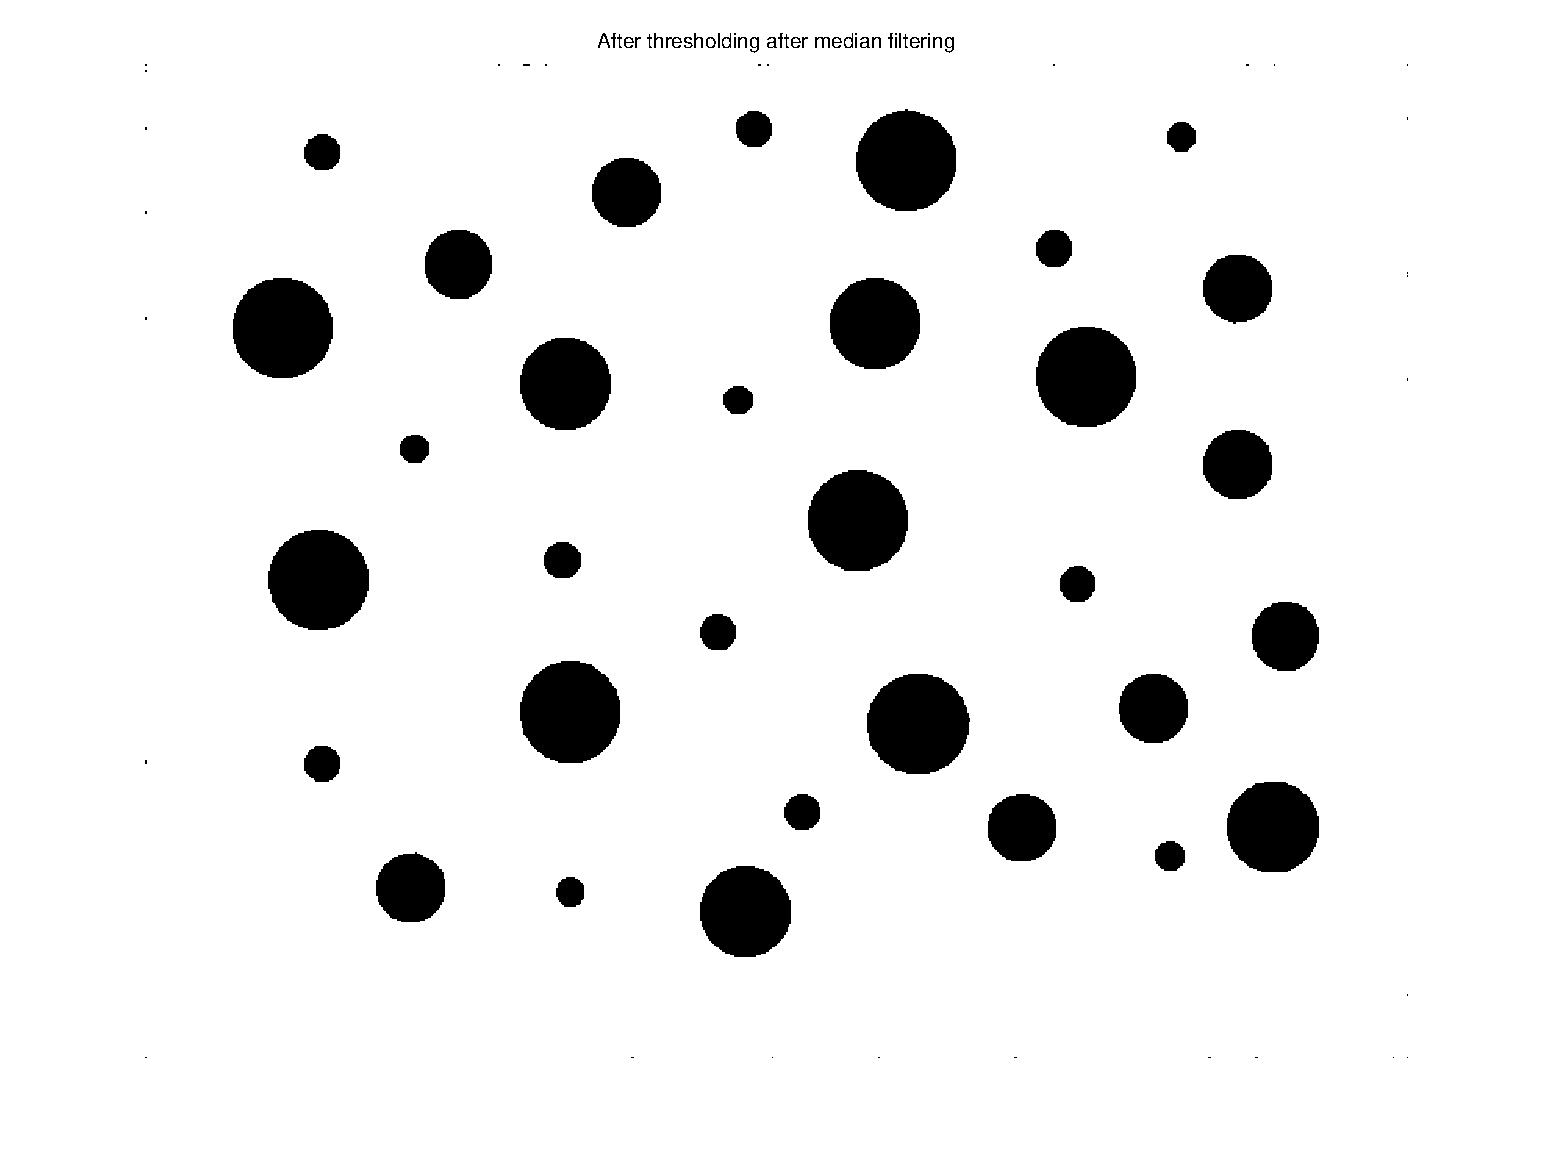
\includegraphics[width=12cm]{AfterThresholdingAfterMedianFiltering.eps}
	\caption{After Thresholding Result.}
	\label{fig:2}
\end{figure}


\subsubsection{Method 2 -  Opening Method (Erosion Is Performed Before Dilation )}

In opening method,  we did the thresholding in the first step. For those pixel value that are larger than 200, we reset the pixel value to 255 (White), and we reset the pixel value to 0 (Black) for those with pixel value smaller than 200.  After thresholding, the pixel value of  salt noise becomes 0, which means the salt noise is removed successfully. The intermediate result is presented in figure \ref{fig:3}. Next, we performed the erosion and then dilation for removing the pepper noise. We chose the structuring element as a disk with diameter 2, which is slightly larger than the pepper noise with diameter 1. Therefore, after we did the erosion on the binary-valued image, the pepper noise disappeared. However, the five different sizes of disks were eroded. Thus, in order to maintain the same shape of the five different sizes of disks scattered on the image, the dilation was necessary to be performed on the result of erosion by using the same structuring element. The result of the opening method is in figure \ref{fig:4}. Apparently, from figure \ref{fig:2} and \ref{fig:4}, we got the same effect for these two methods.
\begin{figure}
	\centering
	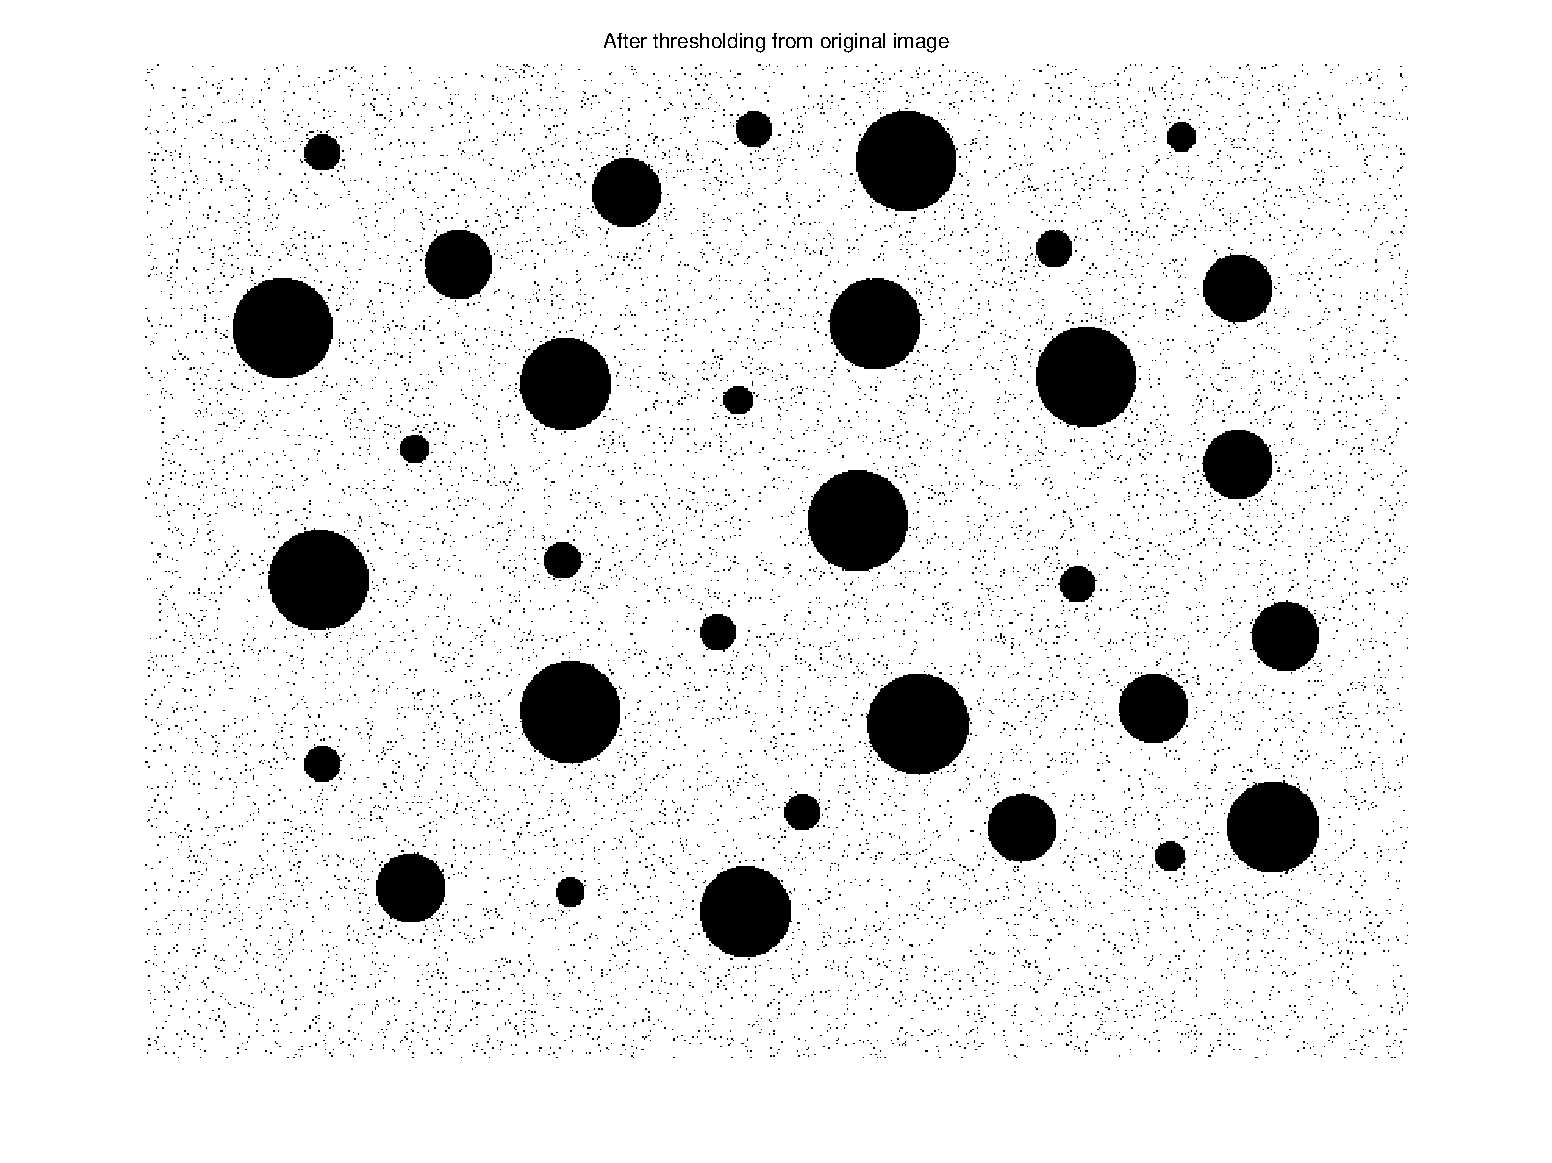
\includegraphics[width=12cm]{threshold.eps}
	\caption{After Thresholding From Input Image}
	\label{fig:3}
\end{figure}

\begin{figure}
	\centering
	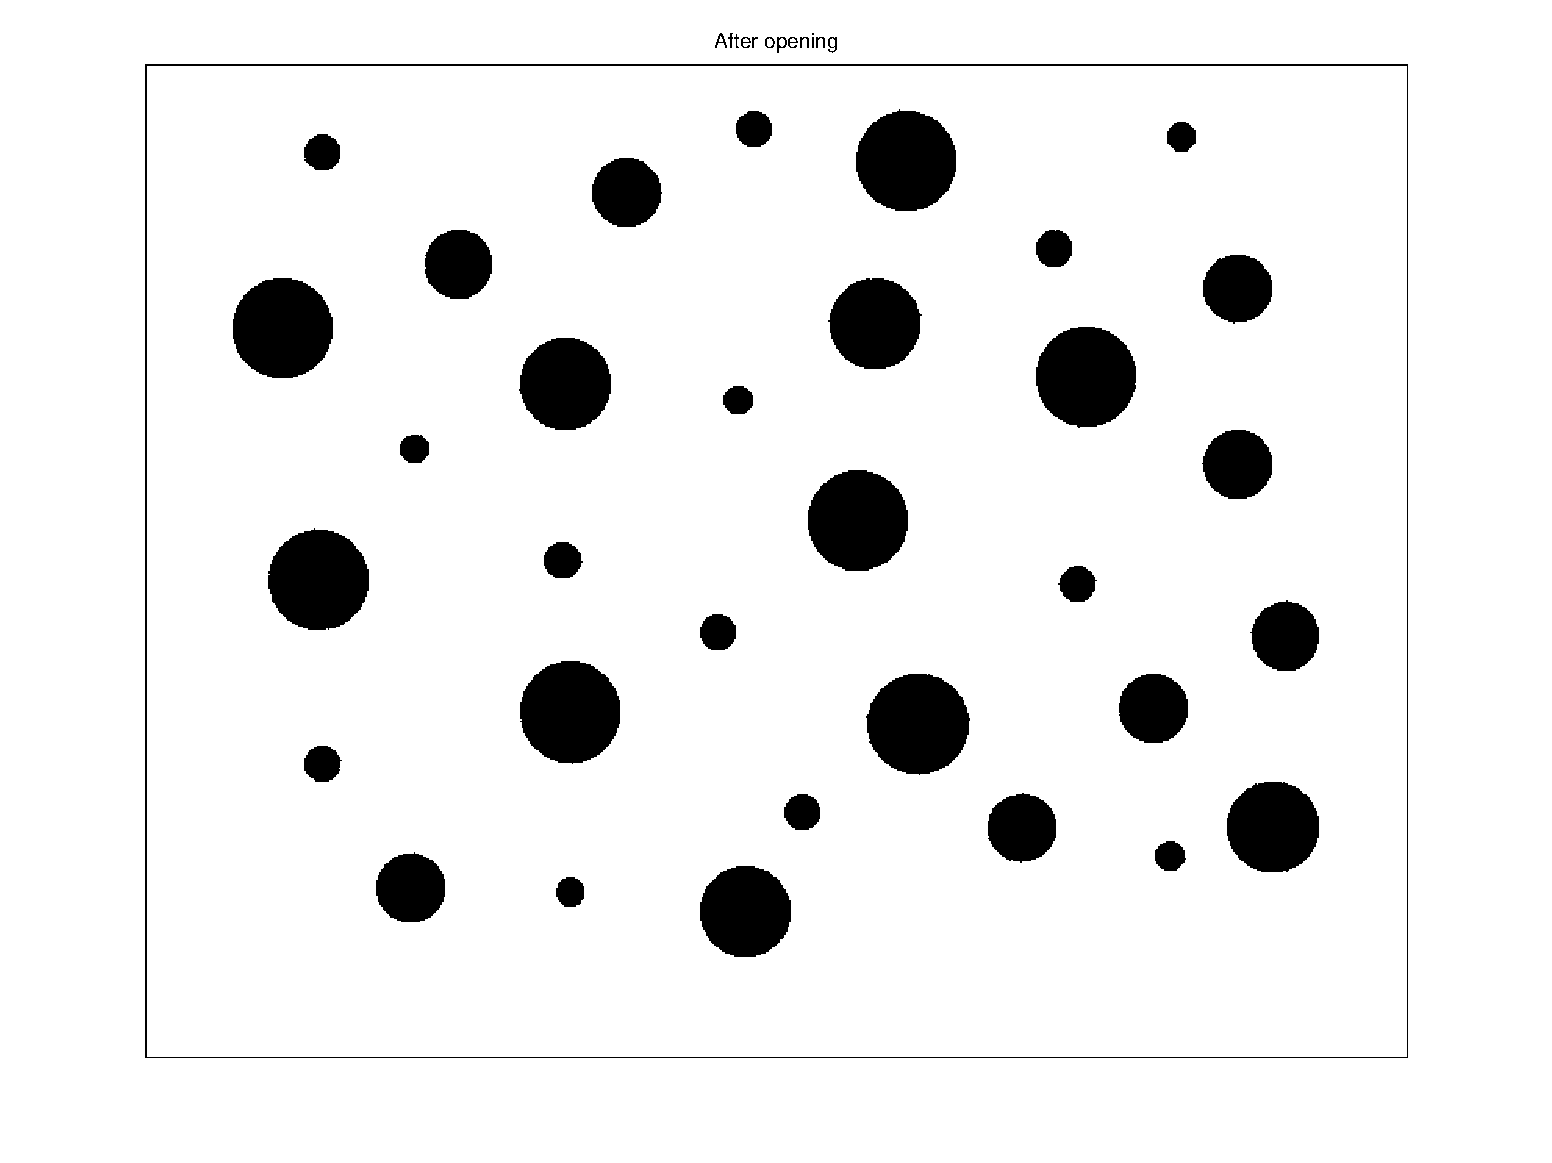
\includegraphics[width=12cm]{opening.eps}
	\caption{Opening Result.}
	\label{fig:4}
\end{figure}





\subsection{Pixel Value Inversion}

For computational convenience, we inverted the value of pixels.  That is, if the grey level is 255, we converted it to 0, and grey level 0 was converted to 255. The result is shown in figure \ref{fig:5}. 
 

\begin{figure}
	\centering
	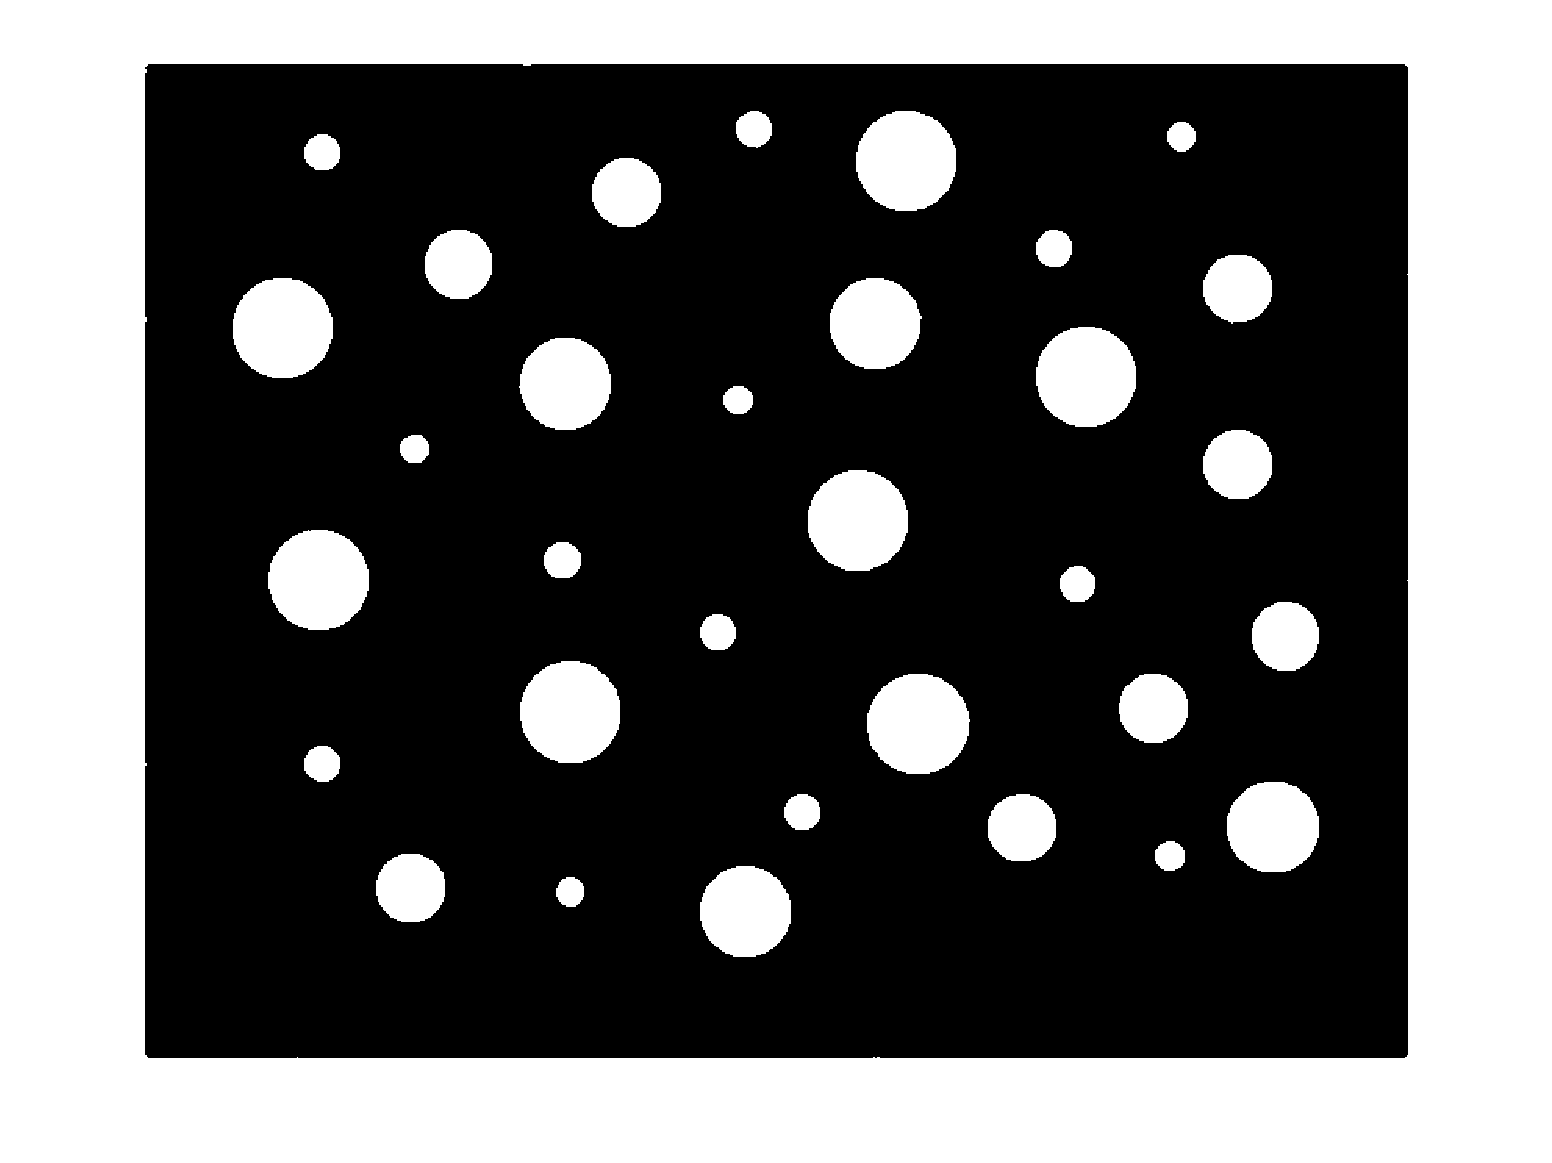
\includegraphics[width=12cm]{complement.eps}
	\caption{Pixel Value Inversion.}
	\label{fig:5}
\end{figure}



\subsection{Hit-or-Miss Transformation}

Because $( X \ominus A^S) - ( X  \oplus  B^S)$ could be derived to $( X \ominus A^S ) \cap (X \oplus  B^S)^c => ( X \ominus A^S) \cap ( X^c \ominus B^S)$, we took the approach in the page 9 of lecture 4 throughout this project1. 

\subsubsection{Structuring Element Selection}

We selected the structuring elements A and B, where B is W - A, and W is the local background of A as presented in the lecture notes. Then, the AND operation was performed with the result of the $( X \ominus A^S )$ and the result of $( X^c \ominus B^S)$. By doing so, we can get the result of the given $( X \ominus A^S) - ( X  \oplus  B^S)$, which is equal to the location of shape A. In other words, in order to locate the location of shape A, we will select A as the structuring element. Clearly, because the goal of this project is to detect the three middle-size disks from the input image, we selected three different structuring elements A for operation $( X \ominus A^S)$ and its corresponding structuring elements W-A (= B) for operation $( X^c \ominus B^S) $.  

In order to detect the second largest disk, we used the first structuring element A1 and B1. A1 is the disk with diameter 57, which is slightly shorter than the diameter of the second largest disk. This is because if we can have a slightly smaller structuring element A1, then the second largest disk can still present after erosion. Obviously, the disks which are larger than the structuring element A1 will be kept after the erosion while the disks which are smaller than the structuring element A1 will disappear.  In addition, the structuring element B1 is supposed to be W1-A1, where W1 is the window with length 65. The length 65 is chosen to cover the structuring element A1. However, in our implementation, we defined the structuring element B1 as W1- A1', where A1' is the hole with diameter 63. The diameter 63 of A1' is slighter larger than the diameter of A1 (57). The reason behind this is similar to what we have done for the structuring element A1. To put in another word, the hole that is larger than A1' will disappear after erosion, and the hole that is smaller than A1' will remain in the image after erosion. Therefore, in order to detect the third largest disk, our structuring element A2 is the disk with diameter 43, and the structuring element B2 is W2-A2', where W2 is the window with length 48 and A2' is the hole with diameter 47. Last, in order to detect the second smallest disk, our structuring element A3 is the disk with diameter  23, and the structuring element B3 is W3-A3', where W3 is the window with length 33, and A3' is the hole with diameter 31. These structuring element's parameters is in $main.m$ file.

\section{Results}

In this section, we present the results of $( X \ominus A^S)$, the result of $( X^c \ominus B^S)$, and the result of $( X \ominus A^S) \cap ( X^c \ominus B^S)$ by using three structuring element A = \{A1, A2, A3.\} and three structuring elements B = \{B1, B2, B3.\} .
Our matlab code can be run by running the $main.m$ file, and the following results will be generated.
\subsection{Structuring Element A1 and B1}

To detect the second largest disk in the input image X, we used the structuring element A1 and B1. A1 is the disk with diameter 57. B1 is W1- A1', where W1 is the window with length 65, and A1' is the hole with diameter 63.

Figure \ref{fig:6} shows the erosion of X by structuring element A1, and figure \ref{fig:7} shows the complemented image $X^c$ eroded by structuring element B1. In figure \ref{fig:8} is the result of the AND operation performed on Figure \ref{fig:6} and Figure \ref{fig:7}. This demonstrates that it detects the location of all the second largest disk in the original input image X.

\begin{figure}
	\centering
	\includegraphics[width=12cm]{SecondBiggestDisk_X_sub_As.eps}
	\caption{ $( X \ominus A1^S)$.}
	\label{fig:6}
\end{figure}

\begin{figure}
	\centering
	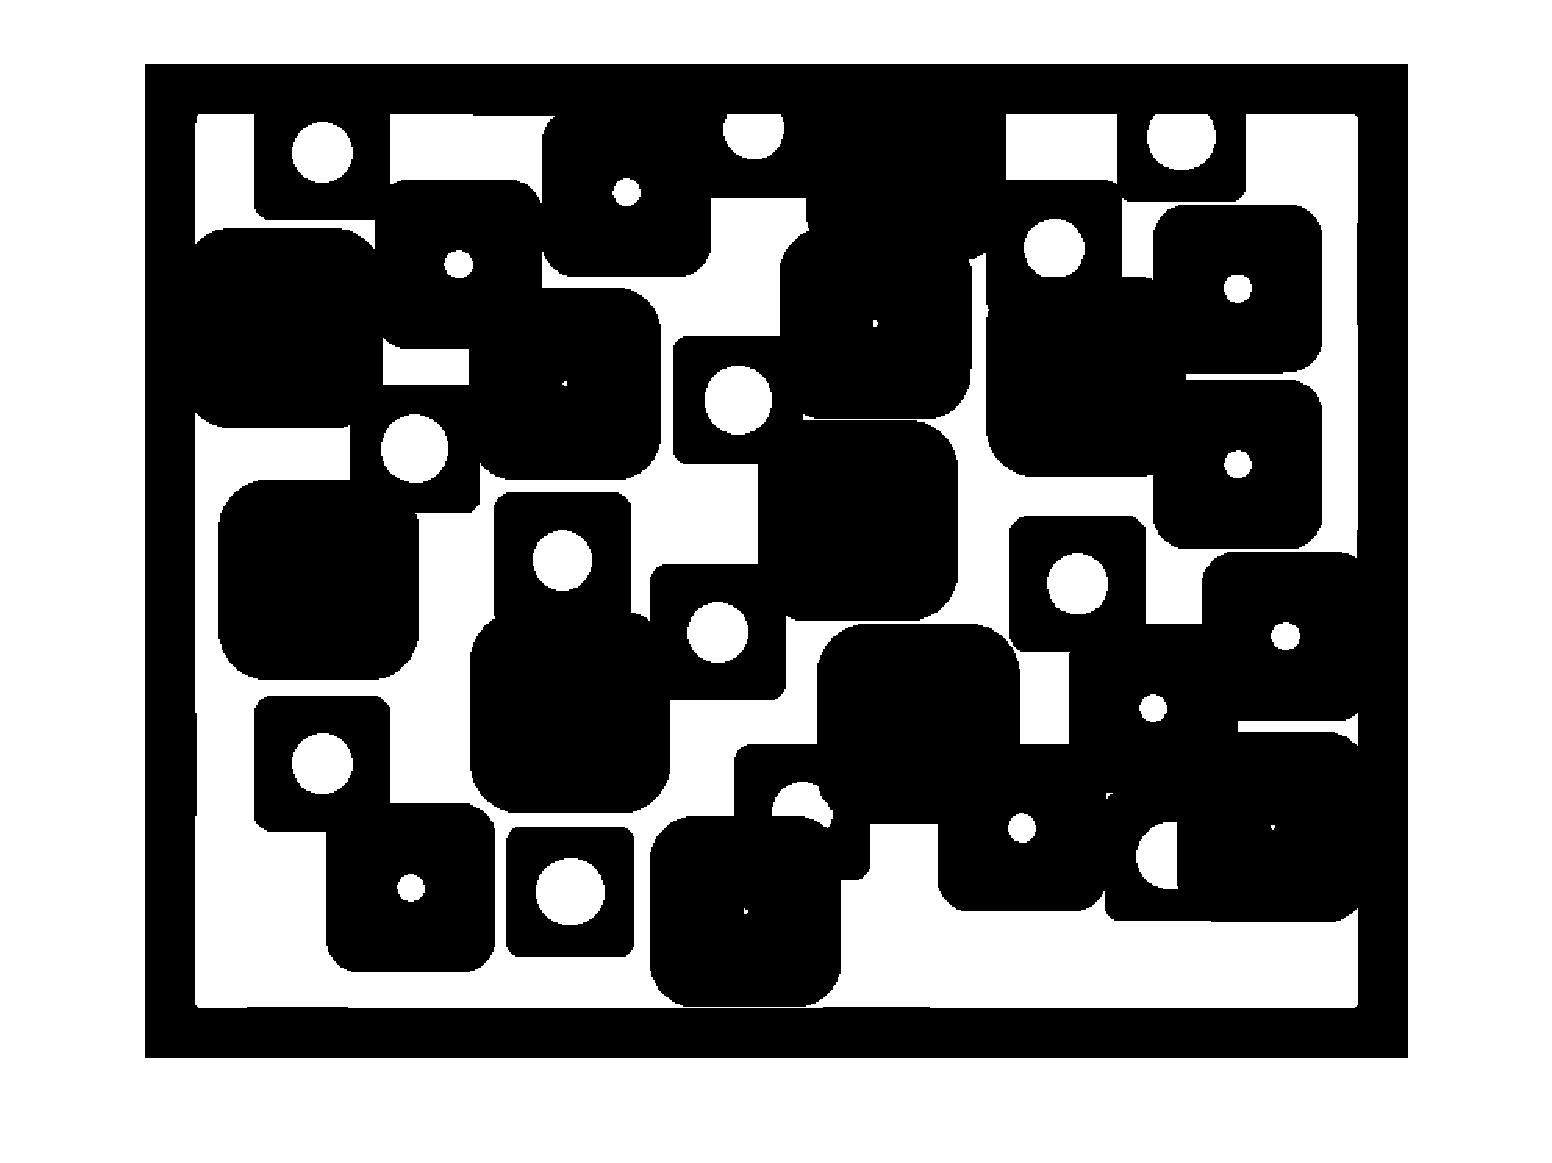
\includegraphics[width=12cm]{SecondBiggestDisk_Xc_sub_Bs.eps}
	\caption{ $( X^c \ominus B1^S)$ .}
	\label{fig:7}
\end{figure}

\begin{figure}
	\centering
	\includegraphics[width=12cm]{SecondBiggestDisk_central_points.eps}
	\caption{ $( X \ominus A1^S) \cap ( X^c \ominus B1^S)$ .}
	\label{fig:8}
\end{figure}


\subsection{Structuring Element A2 and B2}


To detect the third largest disk in the input image X, we used the structuring element A2 and B2. A2 is the disk with diameter 43. B2 is W2- A2', where W2 is the window with length 48, and A2' is the hole with diameter 47.

Figure \ref{fig:9} shows the erosion of X by structuring element A2, and figure \ref{fig:10} shows the complemented image $X^c$ eroded by structuring element B2. In figure \ref{fig:11} is the result of the AND operation performed on Figure \ref{fig:9} and Figure \ref{fig:10}. This demonstrates that it detects the location of all the third largest disk in the original input image X.


\begin{figure}
	\centering
	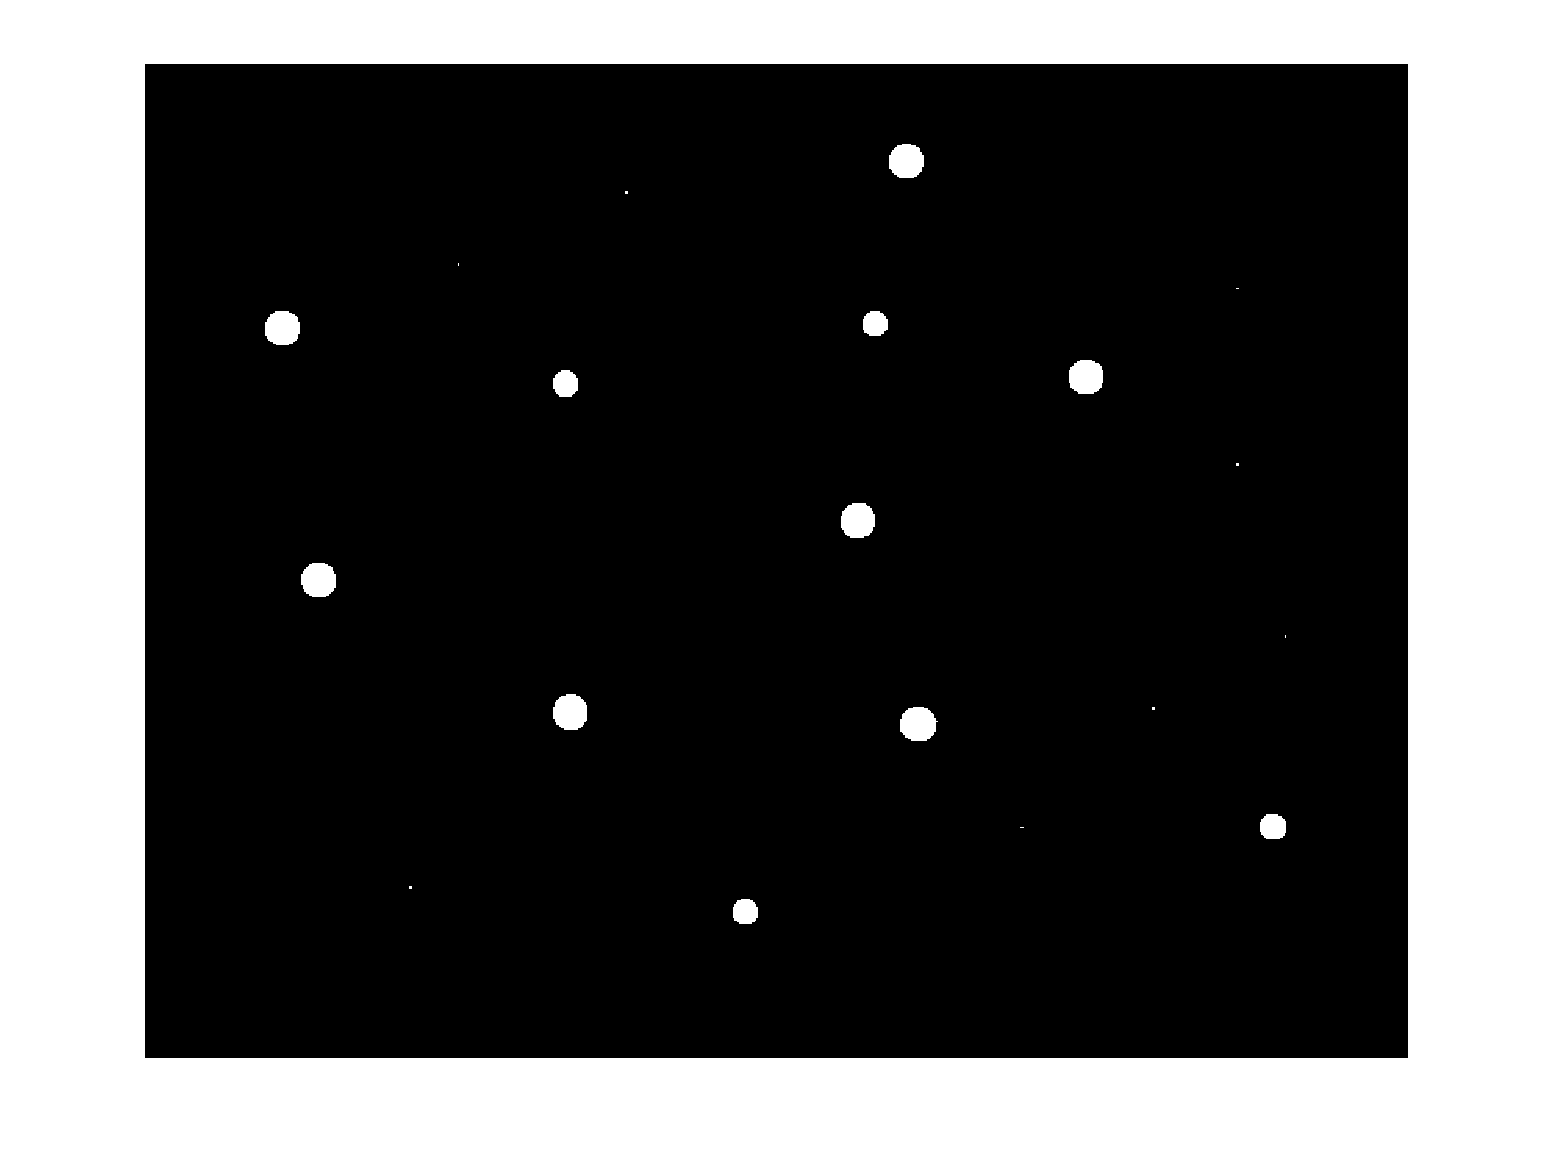
\includegraphics[width=12cm]{MiddleDisk_X_sub_As.eps}
	\caption{ $( X \ominus A2^S)$.}
	\label{fig:9}
\end{figure}

\begin{figure}
	\centering
	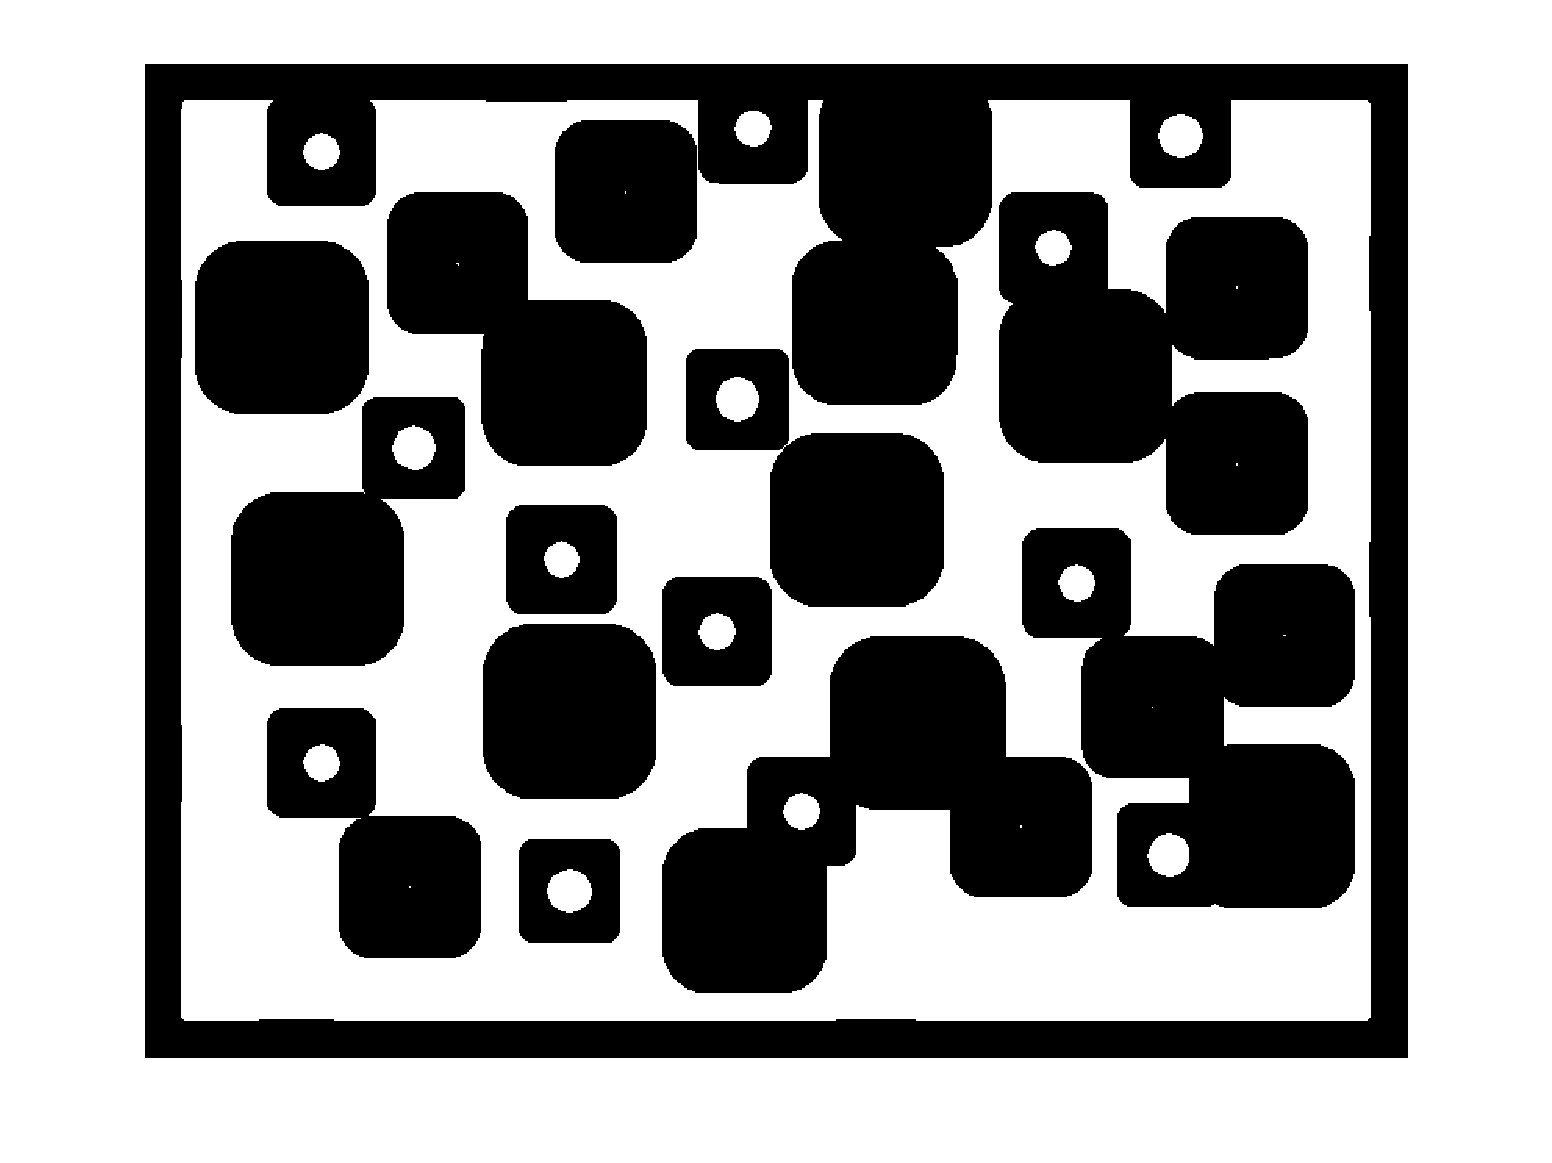
\includegraphics[width=12cm]{MiddleDisk_Xc_sub_Bs.eps}
	\caption{ $( X^c \ominus B2^S)$ .}
	\label{fig:10}
\end{figure}

\begin{figure}
	\centering
	\includegraphics[width=12cm]{MiddleDisk_central_points.eps}
	\caption{ $( X \ominus A2^S) \cap ( X^c \ominus B2^S)$ .}
	\label{fig:11}
\end{figure}






\subsection{Structuring Element A3 and B3}


To detect the second smallest disk in the input image X, we used the structuring element A3 and B3. A3 is the disk with diameter 23. B3 is W3- A3', where W3 is the window with length 33, and A3' is the hole with diameter 31.

Figure \ref{fig:12} shows the erosion of X by structuring element A3, and figure \ref{fig:13} shows the complemented image $X^c$ eroded by structuring element B3. Figure \ref{fig:14} is the result of the AND operation performed on Figure \ref{fig:12} and Figure \ref{fig:13}. This demonstrates that it detects the location of all the second largest disk in the original input image X.







\begin{figure}
	\centering
	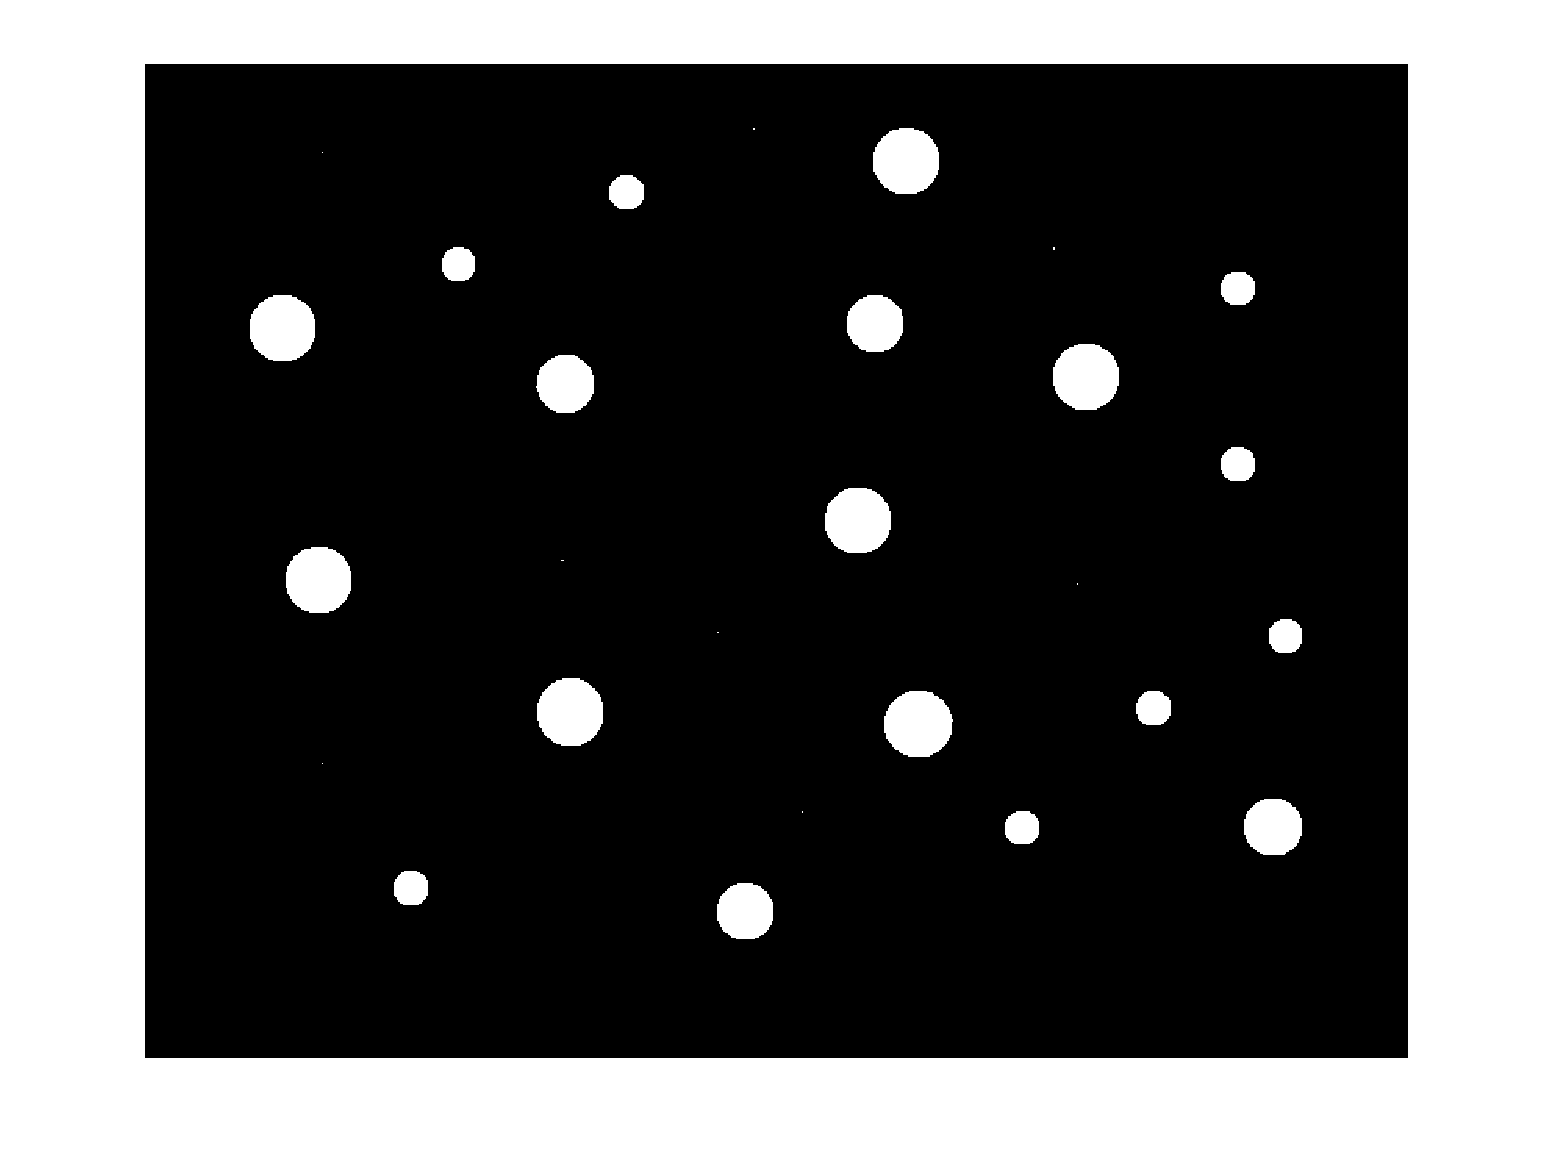
\includegraphics[width=12cm]{XsubAs.eps}
	\caption{ $( X \ominus A3^S)$ .}
	\label{fig:12}
\end{figure}

\begin{figure}
	\centering
	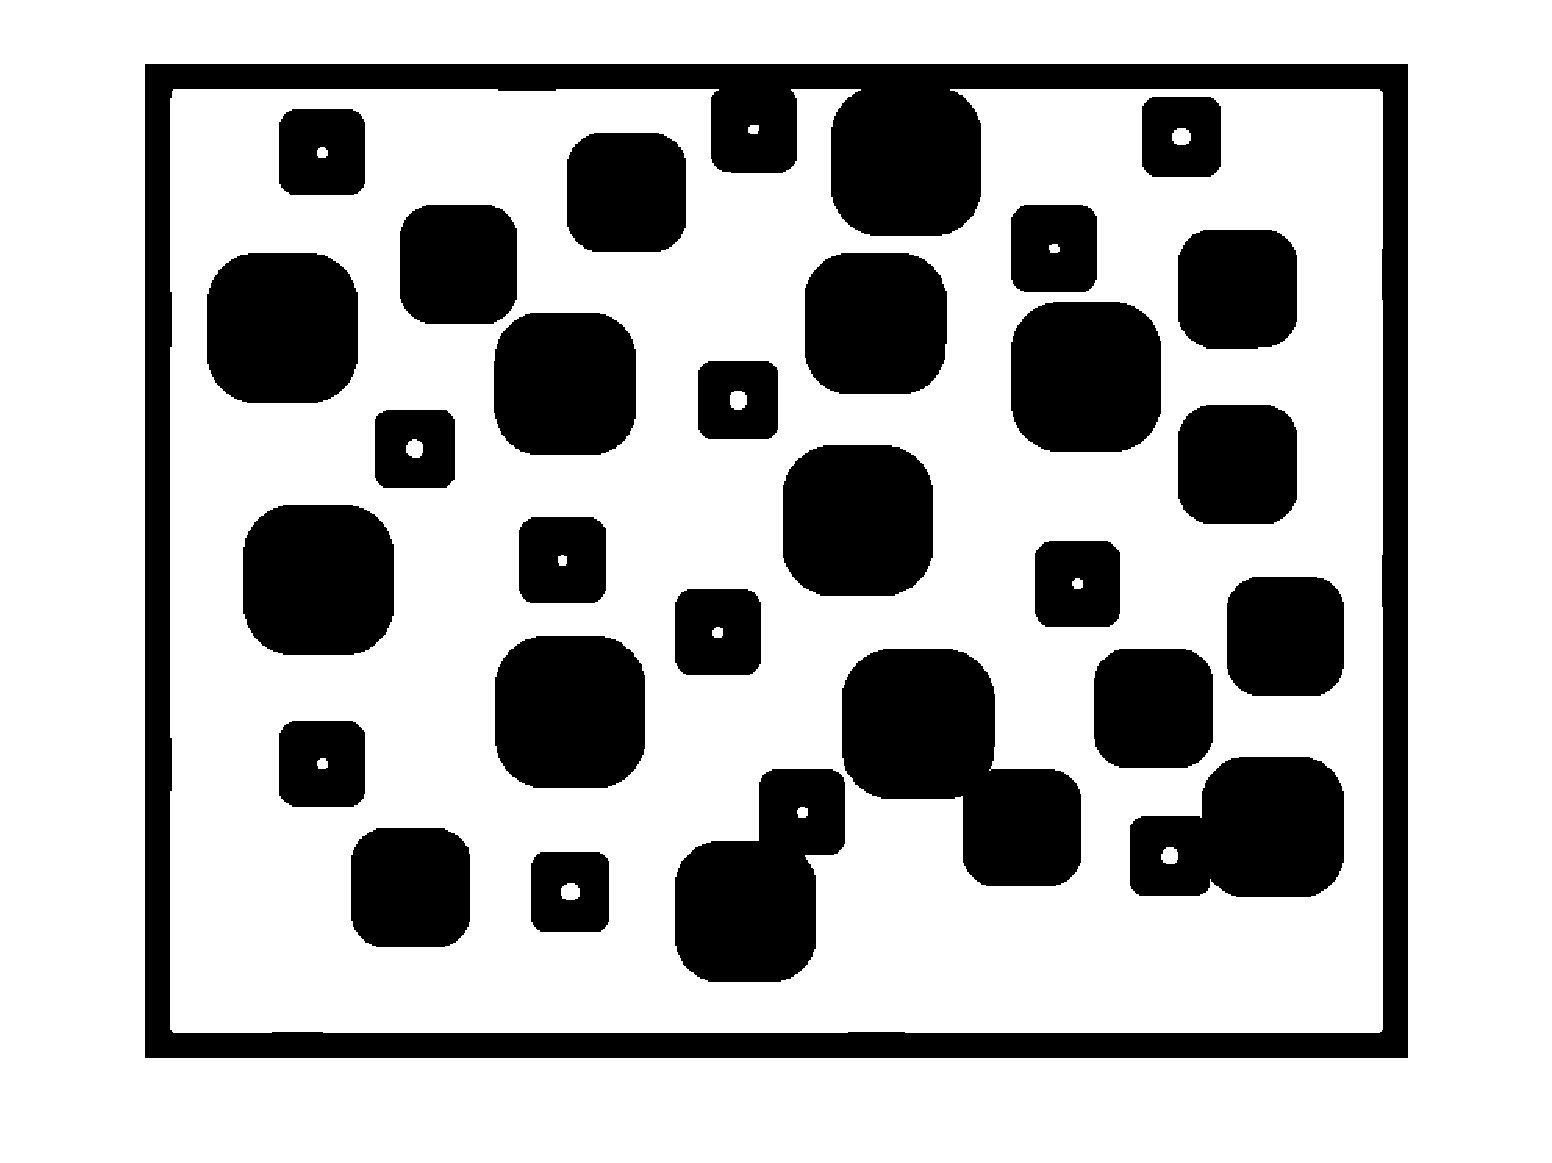
\includegraphics[width=12cm]{XcsubBs.eps}
	\caption{ $( X^c \ominus B3^S)$ .}
	\label{fig:13}
\end{figure}


\begin{figure}
	\centering
	\includegraphics[width=12cm]{andresult.eps}
	\caption{$( X \ominus A3^S) \cap ( X^c \ominus B3^S)$ .}
	\label{fig:14}
\end{figure}

\subsection{Three Middle-Size Disks Location Recognition}
To show the location of three middle-size disks in the same image, the OR operation is conducted on the figure \ref{fig:8}, figure \ref{fig:11}, and figure \ref{fig:14}. As shown in figure \ref{fig:15}, because the gray level value 0(BLACK) OR gray level value 255(WHITE) will give the gray level value 255 (WHITE), we got the white dots which specify the location of all the middle-size disks. In addition, we present the three middle-size disks' location in figure \ref{fig:16}.


\begin{figure}
	\centering
	\includegraphics[width=12cm]{three.eps}
	\caption{Location Of Three Middle-Size Disks.}
	\label{fig:15}
\end{figure}

\begin{figure}
	\centering
	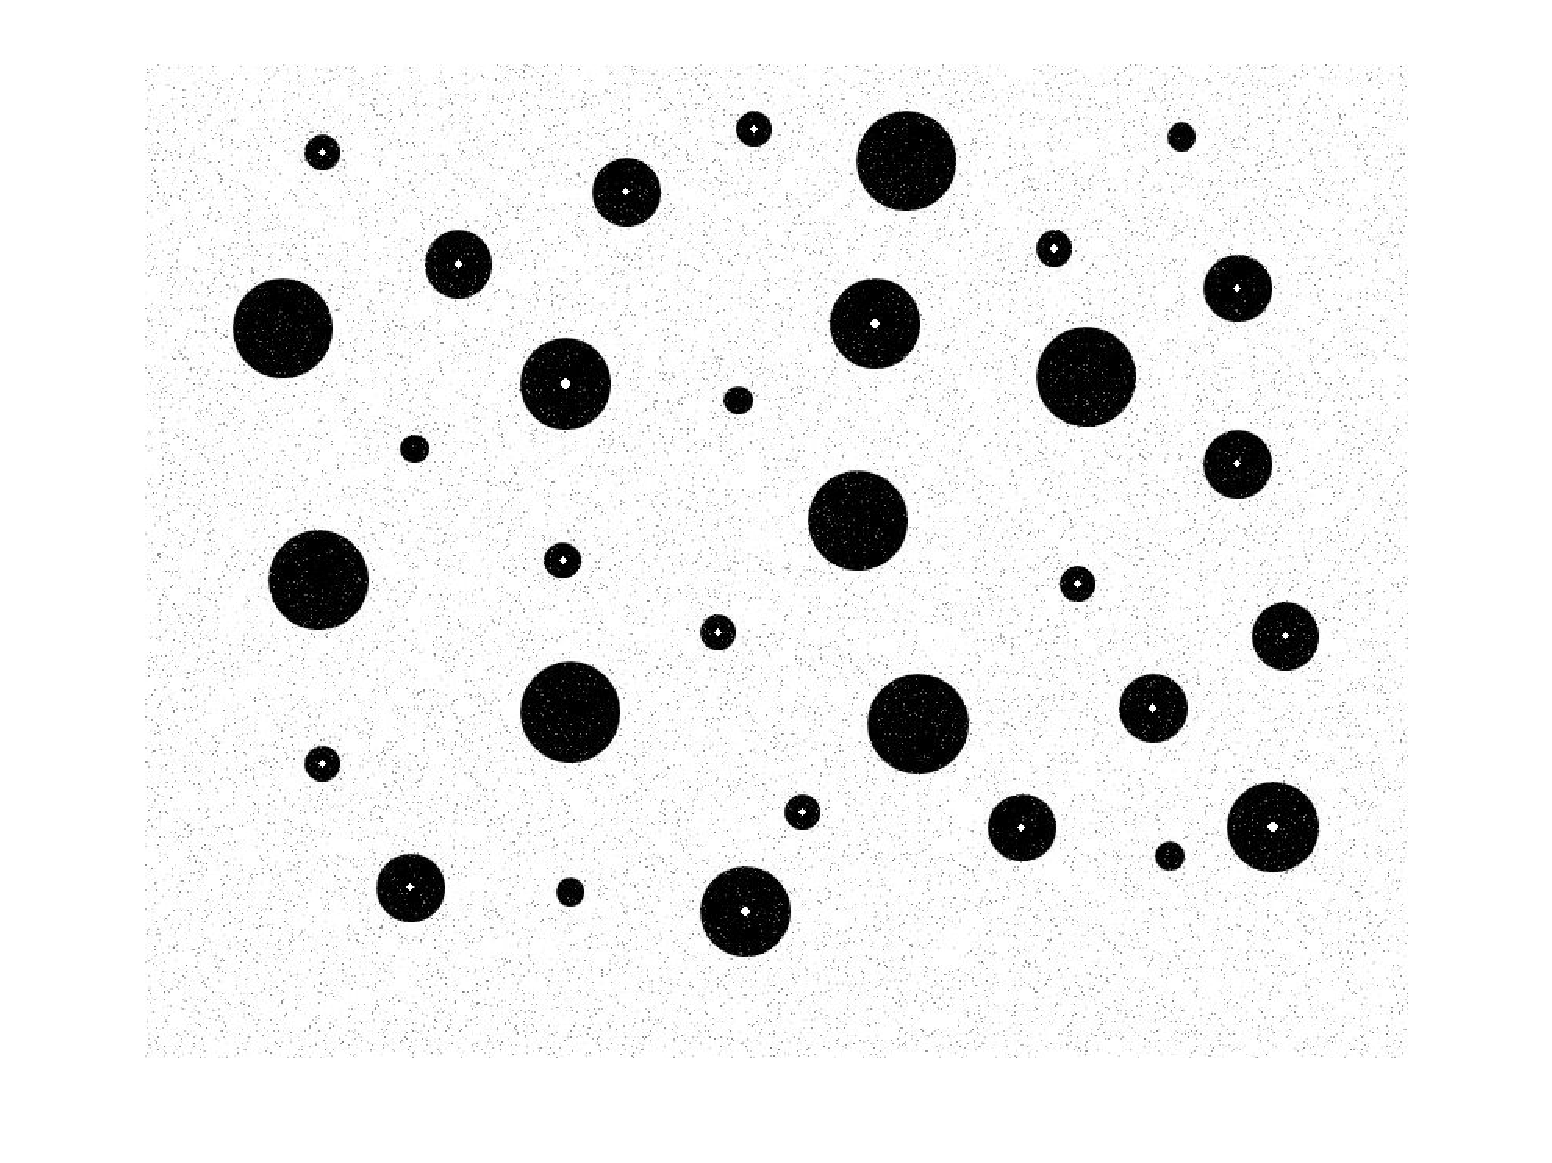
\includegraphics[width=12cm]{Finalresult.eps}
	\caption{Final Result.}
	\label{fig:16}
\end{figure}


\section{Discussion}
In this section, we discuss the situation that we do not apply opening method. In this case, the hit-or-miss transform did not work well. This is because there is still pepper noise in the image after thresholding. For the operation $( X \ominus A^S)$, the result is shown in figure \ref{fig:17}. It is correct because the pepper noise is smaller than the structuring element A and the pepper noise is removed. However, because of the pepper noise, the result of $( X^c \ominus B^S)$ is shown in figure  \ref{fig:18}. Last, the AND operation was performed and the result is presented in \ref{fig:19}, which did not generate the desired results.
\begin{figure}
	\centering
	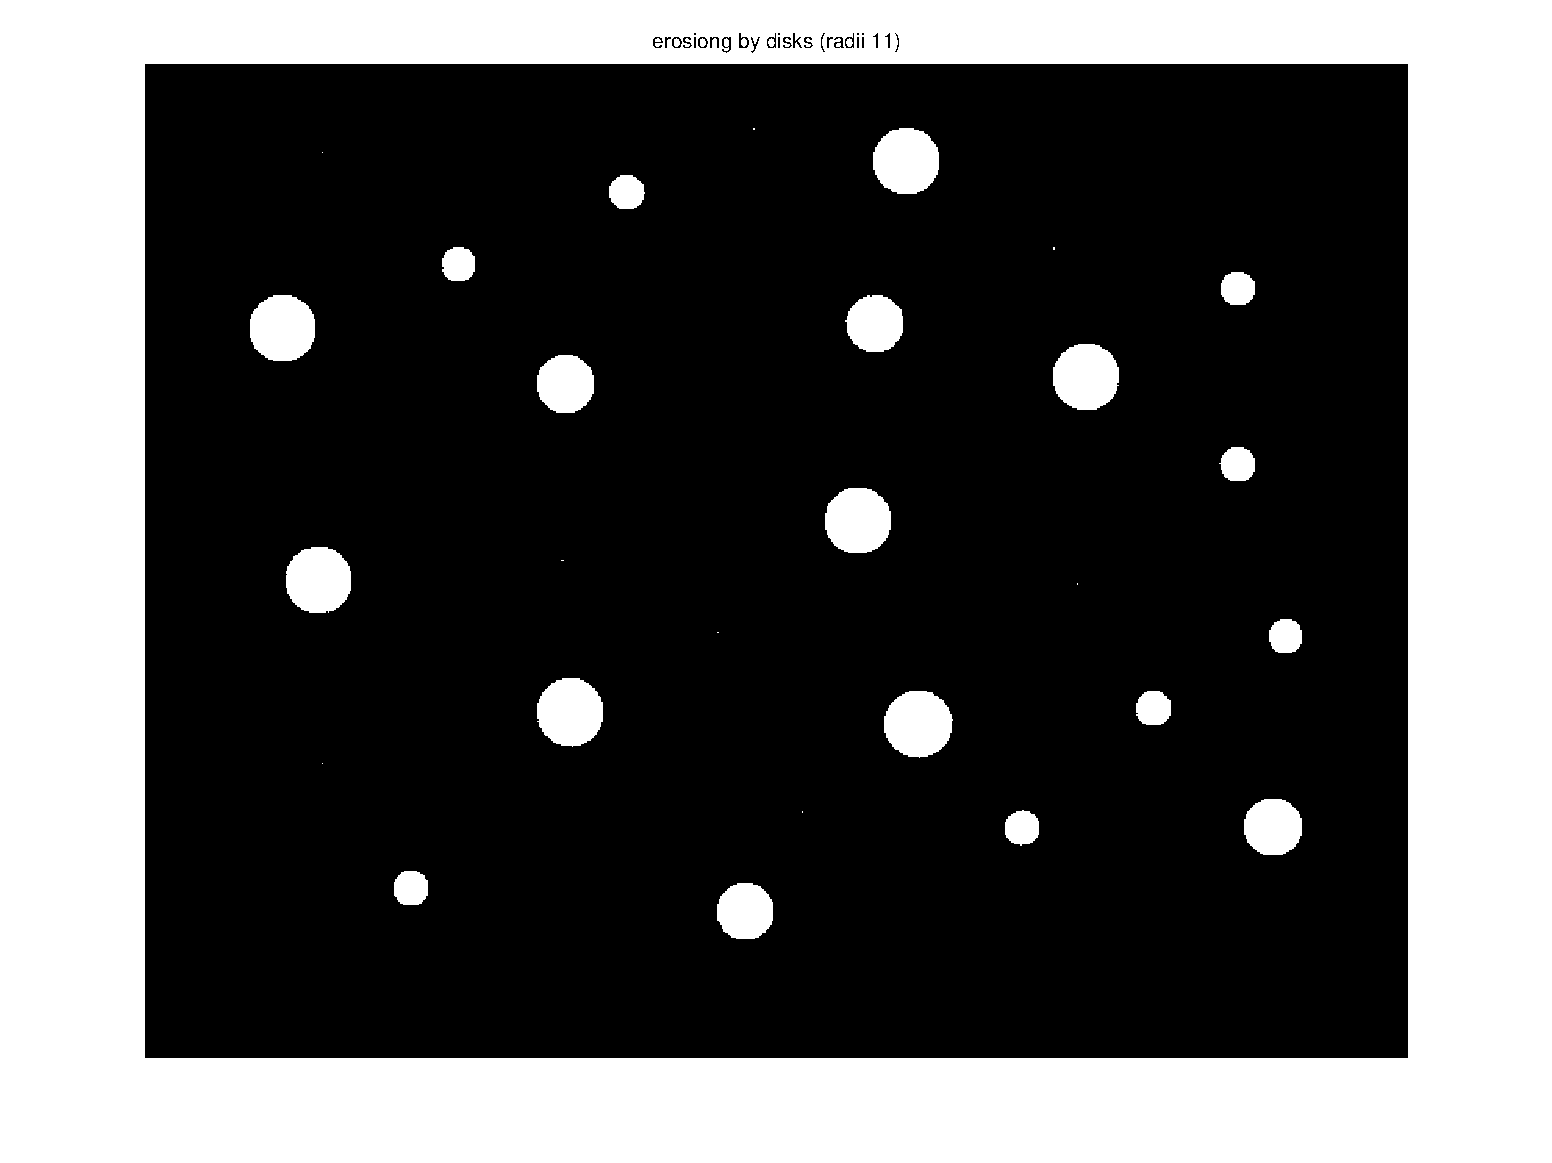
\includegraphics[width=12cm]{D_XsubAs.eps}
	\caption{ $( X \ominus A^S)$ Without Opening Method}
	\label{fig:17}
\end{figure}

\begin{figure}
	\centering
	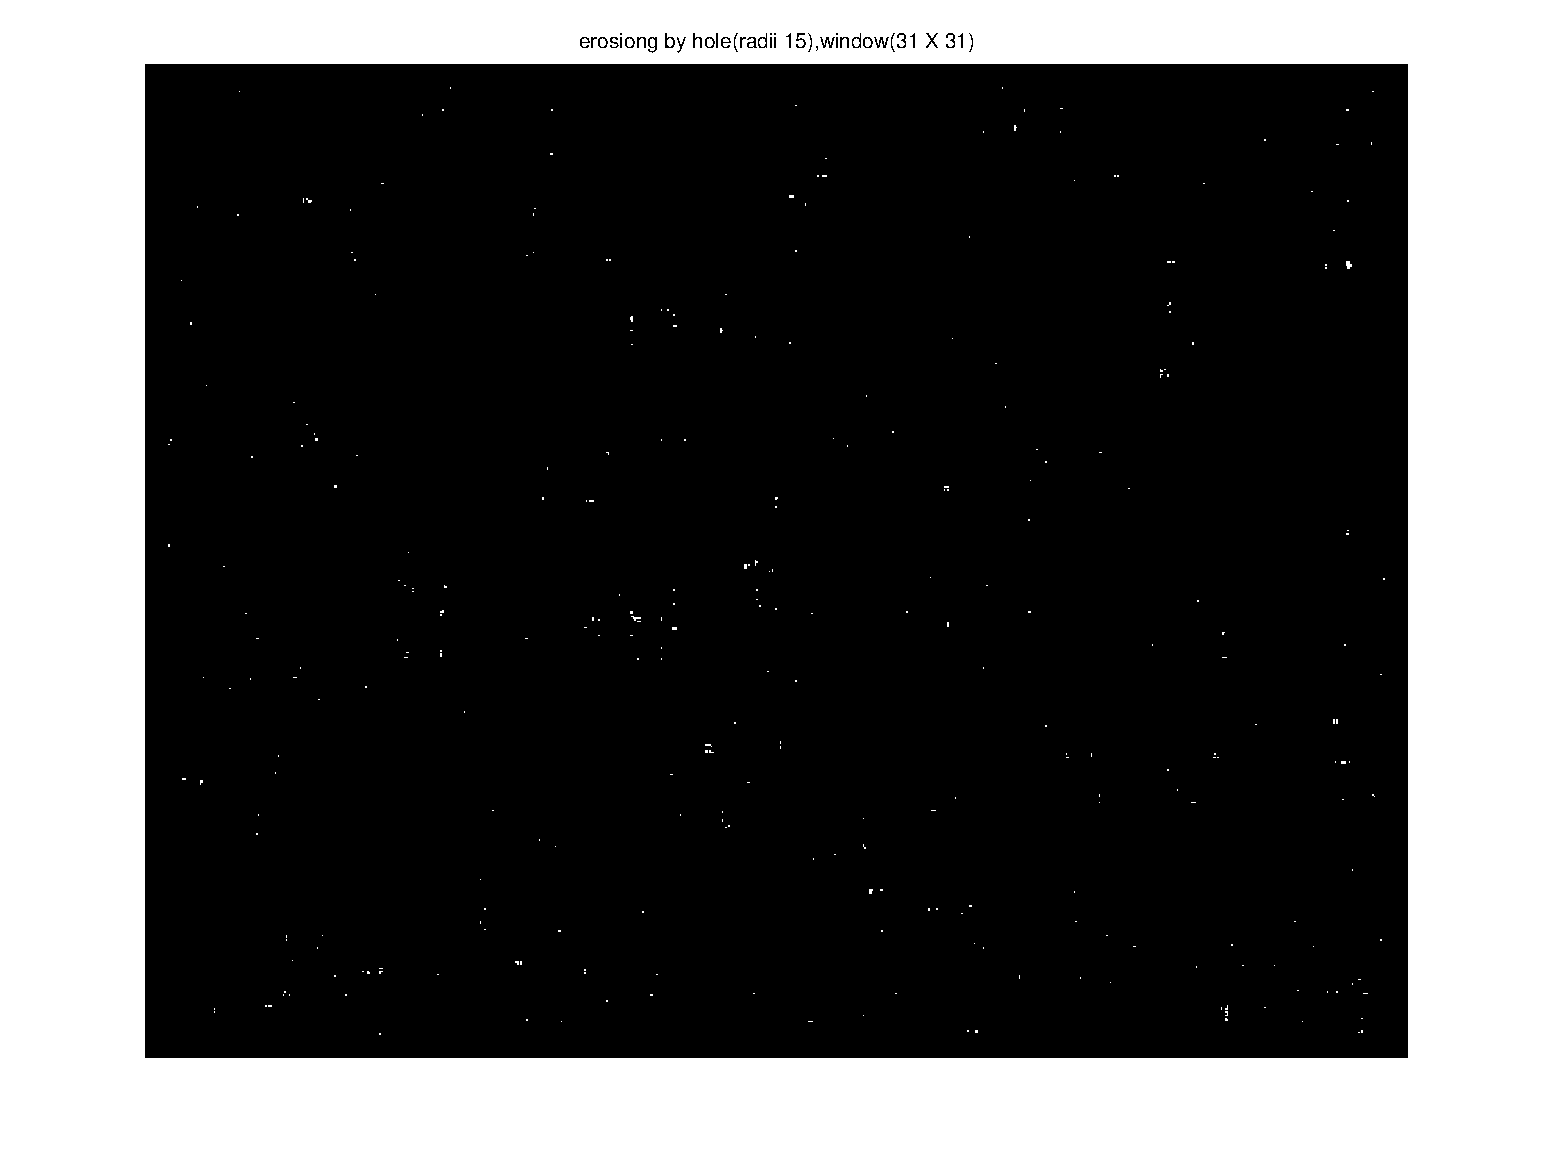
\includegraphics[width=12cm]{D1.eps}
	\caption{ $( X^c \ominus B^S)$ Without Opening Method}
	\label{fig:18}
\end{figure}

\begin{figure}
	\centering
	\includegraphics[width=12cm]{And.eps}
	\caption{ $( X \ominus A^S) \cap ( X^c \ominus B^S)$ Without Opening Method}
	\label{fig:19}
\end{figure}




\section{Conclusion}
To conclude our project, we did noise filtering for image preprocessing. Next, we selected the structuring elements, and applied two hit-or-miss transforms for the given structuring elements A and B. Then, the AND operation on these results helped us to detect a certain size of disk. Finally, we combined three middle-size disks' locations on the same image. Last, the member contributions are shown in Table~\ref{tab:contr}. We also want to thank professor Higgins for his lecture notes and hints.

\begin{table}
	\centering
	\caption{Member Contribution Summary}
	\begin{tabular}{c|c} \hline
       Su, Wei-Kai & experiments \\ \hline
	Kuo, Yu-Hsuan & report \\ \hline
	
	\end{tabular}
	\label{tab:contr}
\end{table}

\end{document}
